\documentclass[12pt]{article}
% New references for this revision live in references-local.bib (auto-loaded by the
% house preamble). Verified against arXiv/Crossref 2026-07-24; PDFs in literature/.
\input{.house-style/preamble.tex}
\usepackage{float}
\usepackage{tikz}
\usetikzlibrary{arrows.meta, positioning, fit}
\hypersetup{
  pdftitle={When Benchmark Inferences Do Not Compose: Projectibility in AI Evaluation},
  pdfkeywords={AI evaluation, benchmark validity, projectibility, construct validity, generalization, AGI}
}
\setlength{\headheight}{14pt}
\setlength{\emergencystretch}{1.5em}

\newcommand{\instab}{\mathrm{INS}}
\newcommand{\wtd}{\mathrm{WTD}}
\newcommand{\wtl}{\mathrm{WTL}}
\newcommand{\Warr}{\operatorname{Warr}}

\title{When Benchmark Inferences Do Not Compose:\\Projectibility in AI Evaluation}
\author{Brett Reynolds \orcidlink{0000-0003-0073-7195}\thanks{I used ChatGPT 5, Claude Sonnet 4.5, and Gemini Pro 2.5 extensively in drafting and revising this paper. I reviewed, edited, and approved all the material and take full responsibility for the final text and conclusions. \href{mailto:brett.reynolds@humber.ca}{brett.reynolds@humber.ca}}\\
Humber Polytechnic \& University of Toronto}
\date{}

\begin{document}

\maketitle

\begin{abstract}
An AI benchmark result rarely reaches a consequential claim in one step. It is generalized to further test cases, interpreted as evidence of a capability, extrapolated to different tasks, transported to a new system or site, and combined with assumptions about human review and downstream consequences. Recent validity-centred approaches correctly require evidence for each claim. This paper identifies a further problem: warranted links don't automatically make a warranted chain. The target of one study may not be the source sampled by the next; the system, population, outcome, or background conditions may change at the interface; and shared data or model lineage may make apparently independent support dependent.

I use \term{projectibility} for the degree of warrant for a bounded extension from observed to unobserved cases. Goodman supplies the problem of rival extensions; argument-based validity supplies the architecture for testing them. The paper's distinctive claim is a non-composition principle: support for adjacent projections warrants their composition only when their endpoints and assumptions align and their dependence and uncertainty are carried through. A worked case involving a legal-research assistant shows how benchmark evidence and a local deployment study can each be sound while remaining parallel rather than composable. A concise reanalysis and simulation show why aggregate stability can erase distinctions that a later projection requires. The resulting projectibility audit complements construct validity, nomological networks, estimands, and causal transportability by specifying when their outputs can be joined.
\end{abstract}

\noindent\textbf{Keywords:} AI evaluation; benchmark validity; projectibility; construct validity; generalization; AGI

\section{The Missing Problem: Composition}\label{sec:introduction}

A benchmark result rarely supports a consequential claim by itself. Consider a common chain of reasoning. A base model scores highly on a multidomain battery. The score is interpreted as evidence of general reasoning. A product built from that model is then expected to perform a professional task. Because a qualified person will review its outputs, the product is expected to improve the final work. That expectation, together with projected savings and an error tolerance, supports authorization. The chain moves among at least five objects: responses to benchmark items, a capability attributed to the base model, outputs from a tool-using application, work after human review, and consequences under a policy. A high score is an observation about the first object. It isn't yet evidence about the last four.

Psychological and educational measurement provide a disciplined response to this problem. On an argument-based view, validity belongs to a proposed interpretation and use of scores, not to a test considered apart from any claim \citep{messick1995Validity,kane2013validating}. Recent work brings that view into AI evaluation. Claim-centred frameworks distinguish measurements, evaluations, and the assertions or decisions drawn from them; construct-validity studies ask whether benchmark content, structure, and relations support the capabilities named; and benchmark-epistemology accounts identify the assumptions needed to move from performance on a learning problem to a scientific conclusion \citep{salaudeen2025measurement,bean2025measuring,freieslebenZezulka2025benchmarking}. These approaches substantially improve on treating a benchmark as valid or invalid without specifying what it is supposed to warrant.

They also make a further problem visible. Evaluation arguments are usually chains, but support for their links doesn't automatically compose. A benchmark may support a claim about new items generated under its rules. A firm may separately show that a particular human--AI procedure works on a sample of its own cases. Both results can be warranted without the first supplying a premise for the second. The local study may bypass the benchmark rather than extend it. Conversely, two studies may appear to meet at a shared noun such as \mention{legal reasoning}, \mention{draft quality}, or \mention{human oversight} while operationalizing different objects, populations, and outcomes. In either situation, adding the studies together doesn't produce the broad claim.

The central claim of this paper is therefore a non-composition principle:
\begin{equation}\label{eq:noncomposition}
\Warr(C_1)\ \land\ \Warr(C_2)
\ \not\Rightarrow\
\Warr(C_2\!\circ C_1).
\end{equation}
Here \(C_1\) and \(C_2\) are adjacent inferential links, not merely two propositions written next to one another. Their composition is warranted only when the cases delivered by the first are the cases sampled or otherwise represented by the second, the object and outcome remain continuous or are linked by new evidence, the assumptions are compatible, and dependence and uncertainty are propagated. Equation~\ref{eq:noncomposition} is not a claim that projections never compose. It states that composition has additional evidential conditions not supplied by warrant for the component links alone.

I use \term{projectibility} for the degree of warrant for one bounded extension from observed to unobserved cases. The term comes from Goodman's treatment of induction, but the account developed here doesn't offer a general solution to induction and doesn't make entrenchment a sufficient condition. It gives a place within a validity argument for a narrower question: exactly what is being projected, across which boundary, under which assumptions, and with what evidence against the differences that could defeat the extension? A \term{projectibility audit} records the answer link by link and then tests whether the links can be composed.

This focus separates the paper from neighbouring proposals without displacing them. A nomological network can make a capability claim more substantive by relating the proposed construct to other constructs and observables \citep{cronbach1955construct,freiesleben2026establishing}. An estimand can state precisely which quantity a study targets \citep{binetteReiter2024estimands}. A selection diagram can identify conditions for transporting a causal effect \citep{pearlBareinboim2014transportability}. Each may supply evidence or structure for a projection. None by itself guarantees that the target of one analysis is the source of the next. Projectibility concerns that boundary-specific warrant and the interfaces among analyses.

The argument proceeds in four stages. Section~\ref{sec:projectibility} locates projectibility within validity theory and distinguishes it from construct meaning, prediction, and decision. Section~\ref{sec:composition} states the interface conditions under which projections can compose and separates composition from convergent and replacement evidence. Section~\ref{sec:legal} works through a legal-research case with a complete sampling rule, defect definition, confirmatory criterion, and hypothetical results that support one projection, defeat another, and leave a third unresolved. Section~\ref{sec:aggregation} then shows why aggregation matters to the philosophical argument: an upstream mean can erase the item-level differences a downstream projection needs to test. Sections~\ref{sec:agi} and \ref{sec:procedure} apply the result to general-capability claims and divide the evidential work between developers and deployers.

\section{Projectibility within a Validity Argument}\label{sec:projectibility}

\subsection{Rival extensions from the same observations}\label{ssec:goodman}

Goodman's new riddle of induction begins with observations that fit incompatible extensions equally well. Every emerald examined before time \(t\) is green. The observations fit the familiar hypothesis that emeralds are green, but they also fit a predicate under which an object is \mention{grue} when it is examined before \(t\) and green or not so examined and blue. The hypotheses agree on every observed emerald and disagree on the next unexamined one. Fit to the source observations therefore doesn't determine which predicate is fit for projection \citep[74--80]{goodman1983}.

The benchmark analogue isn't that evaluators literally invent time-indexed predicates. It is that many classifications of unobserved cases agree on the scored items. Success can be grouped under \mention{general legal reasoning}, under \mention{answering supplied-text legal questions}, under \mention{recognizing patterns in questions drawn from familiar sources}, or under still narrower descriptions. Those predicates may be extensionally equivalent on the test set and diverge on a research request that requires current authority, live retrieval, source comparison, and a cited memo. More observations sampled under the same narrow item-generating rule may distinguish none of them.

Goodman appeals to entrenchment, the history of successful use of a predicate in past projections. Other accounts place more weight on revisable background theory and causal structure \citep[84--98]{goodman1983,boyd1991}. This account needs no single sufficient criterion. Its more modest lesson is that the rule of extension has to be exposed. A target declaration identifies the cases over which rival predicates disagree. Background knowledge identifies differences that could matter. Direct samples, controlled variations, and later observations test those differences. This doesn't remove induction; it makes a particular induction inspectable and revisable.

\subsection{Definition and evidential standing}\label{ssec:definition}

A \term{projection} extends an interpretation, prediction, or explanation from specified source observations to cases not observed in the source study. Its \term{projectibility} is the degree of warrant for that extension relative to a declared target and use. Three restrictions are built into the definition.

First, projectibility belongs to a bounded projective claim, not to a score, benchmark, or system considered in isolation. The same benchmark result may provide substantial warrant for performance on further items generated under a registered template and little warrant for performance on open-ended professional work. Calling the benchmark \mention{projectible} without naming the target suppresses the point at issue.

Second, projectibility is graded but needn't be forced onto one numerical scale. An evaluator may report a predictive estimate and interval, a defeated invariance assumption, an unresolved population gap, and a supported narrow use. Collapsing those into a projectibility score would recreate the aggregation problem this paper diagnoses. The useful statuses are claim-specific: supported to a stated degree, defeated by specified evidence, or unresolved because the relevant evidence is absent or too imprecise.

Third, source fit is only part of the evidence. Warrant for a projection commonly comes from four places. Direct target sampling shows what happens in cases admitted by the target rule. Deliberate variation tests features suspected of changing the result while preserving what the claim treats as invariant. Background knowledge explains why some differences are plausible defeaters and others aren't. Replication across genuinely new levels (another template family, system lineage, site, or period) tests whether an earlier regularity survives the dimension being projected over. None can be replaced by a bare assertion that source and target are similar.

This account belongs inside an argument-based approach to validity. Kane represents a proposed interpretation and use as a sequence of inferences and assumptions, each requiring support commensurate with the ambition of the claim \citep[1--3, 22--25]{kane2013validating}. Messick's unified account likewise treats validity as an evidential judgment about score meaning and use, drawing on content, response processes, internal structure, relations with external variables, and consequences \citep[741--749]{messick1995Validity}. Projectibility names the standing of those parts of the argument that extend beyond cases observed under the source design. It doesn't subsume every validity question. Whether a rubric mis-scores the observed responses is a scoring problem before it is a projection problem; whether a proposed capability has a coherent meaning is an interpretive problem that may condition a projection without being reducible to one.

\subsection{What projectibility adds to neighbouring frameworks}\label{ssec:neighbours}

Recent validity-centred work on AI is close enough that the difference has to be stated precisely. \Textcite{salaudeen2025measurement} offer a claim-aware framework that maps measurements and evaluations to claims, differentiates forms of validity, and recognizes that measurement producers and downstream claimants may be different stakeholders. \Textcite{freieslebenZezulka2025benchmarking} treat predictive benchmarks as measurement tools and specify internal, external, content, consequential, and auxiliary conditions for scientific inferences. \Textcite{bean2025measuring} document construct-validity weaknesses across 445 language-model benchmarks and give practical recommendations for benchmark development. This paper accepts the shared premise: the inferential object is a particular claim, and stronger claims need more evidence.

Its additional object is the \emph{interface between claims}. A claim-centred framework can tell us which evidence would support a benchmark interpretation and which evidence would support a deployment criterion. A projectibility audit asks whether the conclusion of the first is actually a premise of the second. If the benchmark study concerns a base model answering supplied-text questions and the deployment study concerns final memos produced by a retrieval system and reviewed by lawyers, the studies don't meet merely because both are described as legal evaluation. Their evidence may converge on a narrow conclusion, one may replace the need for the other, or they may concern different objects altogether. Composition is a further relation.

The distinction from nomological construct validation is equally important. \Textcite{freiesleben2026establishing} argues that the inferential account provides insufficient resources for articulating the meaning of theoretical capability constructs, and that capability benchmarks should instead be embedded in nomological networks relating tasks, constructs, processes, and external criteria. That objection concerns a use of argument-based validity not made here. This paper neither proposes a meaning for \mention{reasoning} nor infers the possession of reasoning from benchmark scores. It uses Kane's framework for the task it directly addresses: representing a proposed interpretation or use as a sequence of inferences and assumptions whose evidential support can be assessed. A substantive construct attribution, where one is proposed, needs whatever nomological, process, or causal support that attribution requires; the projectibility audit doesn't supply it.

Nor would successful nomological validation remove the composition problem. A nomological network might support an inference from task scores to a reasoning construct, or establish a relation between that construct and an external criterion in a declared population. It wouldn't thereby establish that the relation survives replacement of the benchmarked model by a retrieval-augmented application, that lawyer review catches the application's errors, or that reviewed outputs produce the consequences a deployment policy assumes. Those are further projections over different objects, observations, and conditions. The non-composition result holds whether the construct-attribution link is warranted, unwarranted, or omitted: nomological evidence may warrant one link in a chain, and the principle at issue concerns whether that link joins to the next.

An estimand framework answers another indispensable question: what quantity is the analysis trying to estimate, over which population, under which data-acquisition and aggregation rule? \Textcite{binetteReiter2024estimands} show how benchmark conclusions become confused when those elements are left implicit. A chain may nevertheless require several estimands. One study may estimate an expected score over benchmark items, another a post-review defect probability over local requests, and a third the rate at which defects reach clients. Each can be well specified while the chain remains unsupported because the first quantity doesn't predict the second or the second wasn't sampled under the conditions of the third.

Finally, causal transportability supplies stronger formal results for a narrower kind of projection. Selection diagrams encode differences between source and target domains and establish when a causal relation is identifiable in the target from source experiments and target observations \citep{pearlBareinboim2014transportability}. Projectibility is broader: it covers descriptive generalization, construct interpretation, prediction, explanation, and socio-technical outcomes, and it claims no identification theorem. Where the target claim is causal, a projectibility audit should defer to the corresponding causal requirements rather than treating generic robustness evidence as enough.

Table~\ref{tab:frameworks} summarizes the division of labour. The rows are complementary. The final column identifies the specific question that motivates this paper.

Nothing in the non-composition principle conflicts with Kane's logic. A completely specified interpretation-and-use argument would include the interface assumptions among its inferences, and support for the whole argument would require support for those assumptions. The practical problem in AI evaluation is that the evidence is usually produced in separate studies, by different actors, and later assembled as though favourable conclusions were automatically adjacent. Kane's framework makes room for assumptions at the interfaces among inferences, but it doesn't treat composition as a distinct object of validation. This paper isolates a recurrent failure mode in distributed AI evaluation: separate studies may warrant their own conclusions while differing in the object, population, outcome, conditions, or uncertainty those conclusions need in order to serve as adjacent premises. The projectibility audit makes the interfaces explicit and states the further conditions under which links compose.

\begin{table}[tbp]
\centering\small
\caption{Neighbouring frameworks and the composition question.}\label{tab:frameworks}
\begin{tabular}{@{}>{\raggedright\arraybackslash}p{0.20\linewidth}
                    >{\raggedright\arraybackslash}p{0.25\linewidth}
                    >{\raggedright\arraybackslash}p{0.27\linewidth}
                    >{\raggedright\arraybackslash}p{0.20\linewidth}@{}}
\toprule
Framework & Primary object & Question answered & Further composition question \\
\midrule
Argument-based validity & Interpretation-and-use argument & Which assumptions and evidence support a stated interpretation or use? & Does one supported conclusion supply the premise required by the next link? \\
Nomological network & Construct and its theoretical and empirical relations & What gives a capability construct content, and do its predicted relations hold? & Do those relations survive a change of task, system, site, or time? \\
Estimand specification & Metric, population, data acquisition, and aggregation & Which quantity does this analysis estimate? & Are the estimands at adjacent links defined over aligned cases and outcomes? \\
Causal transportability & Causal relation across source and target domains & Under which assumptions is a target causal effect identifiable? & Are later interpretive, workflow, or decision links also supported? \\
Projectibility audit & Specified extension and its interfaces & What warrants this source--target extension, and can it be joined to adjacent extensions? & The question is explicit rather than presumed. \\
\bottomrule
\end{tabular}
\end{table}

\section{Why Warranted Links Don't Automatically Compose}\label{sec:composition}

\subsection{Typed nodes and projection edges}\label{ssec:typed}

The easiest way to conceal an inferential gap is to give both sides the same broad noun. A benchmark contains \mention{legal tasks}; a firm performs \mention{legal tasks}; therefore the score is said to transfer. A developer tests \mention{the model}; a deployer uses \mention{the model}; therefore the tested and deployed objects are treated as continuous. A projectibility audit replaces those nouns with typed descriptions.

For an empirical node in an evaluation argument, let
\begin{equation}\label{eq:node}
N=\langle O,P,C,Y,t\rangle,
\end{equation}
where \(O\) is the object tested, \(P\) the population or case-generating rule, \(C\) the operating conditions, \(Y\) the observation or outcome recorded, and \(t\) the period or version. In a benchmark node, \(O\) might be a named model build; \(P\) the held-out items produced under specified templates; \(C\) the prompt, decoding, tool access, and scorer; \(Y\) item correctness; and \(t\) the evaluation date. In a deployment node, \(O\) might instead be a model, retrieval index, prompt stack, and lawyer-review procedure; \(P\) a rule admitting two kinds of logged research request; \(C\) the firm's database and review instructions; \(Y\) a substantive defect remaining in the final memo; and \(t\) the next six months.

Not every node is itself an empirical population. A construct interpretation such as \mention{general reasoning} has theoretical content rather than a sampling frame. It can still be typed by stating the performances, contrasts, and relations that would count for or against it. A nomological network does this work. The important constraint is that the node resolve into commitments that can meet another node: which systems possess the attributed capacity, which behaviours manifest it, and under which conditions the relation is expected to remain stable.

A projection edge \(e:N_s\rightsquigarrow N_t\) consists of a target claim, assumptions \(A_e\) that connect the source and target, and evidence \(E_e\) bearing on those assumptions. Generalizing from observed benchmark items to further items under the same generating rule is one edge. Interpreting the resulting score as evidence of a capability is another. Extrapolating to a new task population, transporting a relation to a new model build, and predicting a post-review outcome are further edges. The notation forces no commitment that every argument has the same sequence. It prevents an argument from treating a sequence as one undifferentiated leap.

Figure~\ref{fig:chain} shows a common evaluation chain. The labels below the arrows name evidence that can answer each link. No amount of evidence under one arrow automatically fills another.

\begin{figure}[tbp]
\centering
\footnotesize
\resizebox{\linewidth}{!}{%
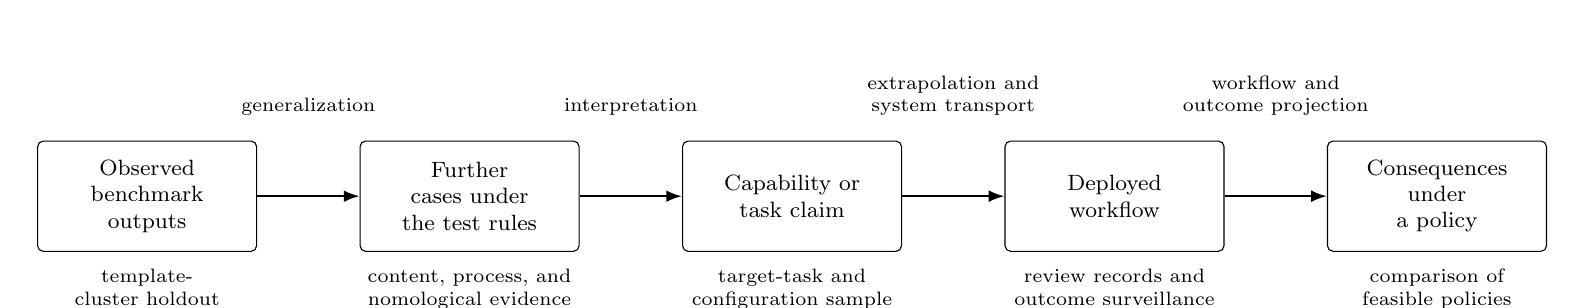
\begin{tikzpicture}[
  node distance=5.5mm,
  box/.style={draw, rounded corners=2pt, align=center, inner sep=4pt,
              text width=25mm, minimum height=14mm, font=\footnotesize},
  flow/.style={-{Latex[length=2mm]}, thick},
  lab/.style={align=center, font=\scriptsize, text width=28mm}
]
\node[box] (obs) {Observed\\benchmark outputs};
\node[box, right=13mm of obs] (uni) {Further cases under\\the test rules};
\node[box, right=13mm of uni] (con) {Capability or\\task claim};
\node[box, right=13mm of con] (app) {Deployed\\workflow};
\node[box, right=13mm of app] (out) {Consequences under\\a policy};

\draw[flow] (obs) -- node[lab, above=9mm] {generalization} (uni);
\draw[flow] (uni) -- node[lab, above=9mm] {interpretation} (con);
\draw[flow] (con) -- node[lab, above=9mm] {extrapolation and\\system transport} (app);
\draw[flow] (app) -- node[lab, above=9mm] {workflow and\\outcome projection} (out);

\node[lab, below=1mm of obs.south] {template-cluster holdout};
\node[lab, below=1mm of uni.south] {content, process, and nomological evidence};
\node[lab, below=1mm of con.south] {target-task and configuration sample};
\node[lab, below=1mm of app.south] {review records and outcome surveillance};
\node[lab, below=1mm of out.south] {comparison of feasible policies};
\end{tikzpicture}%
}
\caption{A benchmark-to-use argument as a chain of typed claims. Evidence is matched to the arrow it supports. A warranted path requires both warranted links and warranted interfaces among them.}\label{fig:chain}
\end{figure}

\subsection{Six interface conditions}\label{ssec:interfaces}

Suppose \(e_1:N_0\rightsquigarrow N_1\) and \(e_2:N_1'\rightsquigarrow N_2\) are each supported. Their composition requires more than the verbal resemblance of \(N_1\) and \(N_1'\). Six interface conditions are especially common.

\emph{Endpoint alignment.} The target reached by the first link must be the source represented in the second, or a further mapping has to be supported. A result about supplied-text questions doesn't arrive at a population of live-retrieval requests. A score interpreted as a latent capability doesn't arrive at a measured defect rate unless the capability--criterion relation has been tested.

\emph{Object continuity.} A base model, a model connected to a database, a complete application with citation validation, and a memo after lawyer review are different objects. Evidence about one can bear on another, but only through a declared system or workflow projection. Product names and version families don't establish continuity. Shared training, distillation, retrieval components, or evaluation data may create dependence without preserving behaviour.

\emph{Population alignment.} The cases reached by the upstream projection must have the distribution, support, and grouping assumed downstream. A study on short, self-contained questions doesn't supply cases for a study whose source consists of open-ended requests with disputed authorities. Even within one task label, a downstream study may sample routine files while the upstream claim includes novel, urgent, or multilingual work. The inclusion rule, not the label, determines alignment.

\emph{Outcome and scale continuity.} The first edge must deliver the quantity the next edge uses. Benchmark accuracy, a factor score, the probability of a citation defect in a draft, a defect after review, and a client loss are not interchangeable outcomes. Mapping all of them to \([0,1]\) doesn't give equal differences equal meaning. If the outcome changes, the mapping itself is an inferential link.

\emph{Condition and assumption compatibility.} Assumptions that support one edge can fail under the conditions of the next. Review may reduce one error class while increasing delay or inducing overreliance; retrieval may improve source coverage while introducing irrelevant but persuasive cases. Relevant effect modifiers have to be carried to the interface rather than averaged away. Two studies conducted under incompatible prompts, databases, reviewer instructions, or time horizons don't compose without evidence that those differences are harmless for the target claim.

\emph{Dependence and uncertainty propagation.} A chain can look better supported than it is when its links reuse the same items, scorer, model lineage, or development decisions. Twenty outputs from one build aren't twenty systems, and thirty-two comparisons among related models and shared benchmarks aren't thirty-two independent replications. Where estimates are composed, their covariance, selection, and uncertainty must be represented. Where a qualitative assumption is uncertain, the chain inherits that uncertainty rather than resetting to certainty at the next arrow.

These conditions are jointly demanding because composition is a stronger conclusion than either component. A simple probability identity makes the point. Let \(B\) be a benchmark result, \(D\) a draft-level outcome, and \(Z\) a final outcome after review. In a target population \(T\),
\begin{equation}\label{eq:composition_identity}
P_T(Z\mid B)
  =\sum_d P_T(Z\mid D=d,B)\,P_T(D=d\mid B).
\end{equation}
A study estimating \(P_{S_1}(D\mid B)\) in one system population and another estimating \(P_{S_2}(Z\mid D)\) in another doesn't identify the terms on the right of Equation~\ref{eq:composition_identity}. The benchmark relation may change in the deployed configuration; review effectiveness may depend on request type or on information not contained in \(D\); and the two source populations may differ from \(T\). Formal causal claims require still stronger conditions, but the identification failure arises even for a descriptive prediction.

\subsection{Composition, convergence, and replacement}\label{ssec:relations}

Three relations among studies are easily conflated. In \term{composition}, the conclusion of one study supplies a premise or population for the next. A benchmark score predicts draft defects across systems; draft defects predict post-review defects under a specified procedure; those links may be composed if their systems, cases, outcomes, and conditions align.

In \term{convergence}, distinct evidence bears on the same claim without forming a chain. A benchmark, expert assessment, and process intervention might each support a reasoning attribution. Their agreement can strengthen the claim, but no result is passed as an input from one study to another. Dependence still matters: three tests built from the same source materials don't provide three independent routes.

In \term{replacement}, direct target evidence makes an ambitious upstream projection unnecessary for a narrower purpose. A firm that samples its own research requests and measures final reviewed defects can assess that workflow without first proving that the base model possesses general legal reasoning. The local study doesn't validate the generality of the benchmark. It starts from new source observations closer to the target. This is often epistemically preferable: direct target evidence can support a bounded policy while the capability question remains open.

The distinctions matter because the phrase \mention{benchmark plus local validation} can describe all three. If the local study compares several systems and tests whether their benchmark profiles predict their defect rates on the same requests, it tests a composable predictive edge. If it evaluates only one frozen application, the benchmark profile is constant across its requests and can't explain which request fails. The local study then replaces, rather than confirms, the benchmark-to-use projection. If both studies are cited merely because they sound favourable, they provide neither composition nor well-characterized convergence.

\subsection{A concrete counterexample}\label{ssec:counterexample}

Consider two individually true claims. First, a model answers 90\% of held-out supplied-text legal questions correctly under the benchmark protocol. Second, lawyers following a written review instruction catch 99\% of fabricated citations in drafts generated for a set of routine research requests. Neither result is defective on its own. Their conjunction still doesn't warrant that reviewed memos are substantively correct.

The retrieval system may omit controlling authority without fabricating any citation. The benchmark never tests retrieval, and the review study counts only fabricated citations. Suppose the application omits a controlling case on 20\% of requests, the omission is not visible from the citations that remain, and the lawyers' procedure doesn't require an independent update search. Both premises remain true while one fifth of final memos contain a substantive defect. The chain fails at two interfaces: the outcome changes from supplied-text correctness to citation fabrication, and the review evidence doesn't cover omitted authority. Adding the two percentages obscures rather than repairs the gap.

The counterexample also shows what positive evidence would look like. The firm could prepare an authority list independently of the system, score omitted controlling authority as well as citation fabrication, and require reviewers to compare every final memo with that list or conduct a defined update search. The revised study would not make the benchmark general. It would supply observations for the missing workflow link.

\section{A Worked Projectibility Audit}\label{sec:legal}

\subsection{The source result and the proposed use}\label{ssec:legal_setup}

Suppose a developer reports a high legal-reasoning score for a base model. The battery presents each question with a fixed set of materials and marks the answer against a reference response. Its held-out design may support generalization to further questions produced under the same item rules. The score doesn't observe whether the model can find current law, distinguish controlling from merely similar authority, produce a linked citation, or work within a lawyer's review procedure.

An Ontario employment-law group is considering a product built from the model. The application receives a lawyer's research request, searches the firm's licensed legal database, and drafts a one-page memo. The firm proposes to authorize it only for two kinds of request: whether a termination clause is enforceable and what period of reasonable notice is likely. An eligible request is written in English, concerns Ontario law, identifies the relevant dates and employment facts, and asks one of those two questions. Requests concerning another jurisdiction, a different subject, missing facts that prevent research, or a novel constitutional issue are outside the target. Each memo must identify the issue, state the governing propositions, cite the current controlling authorities, link each proposition to a passage that supports it, and undergo line-by-line lawyer review before it leaves the firm.

The object under consideration is therefore not the benchmarked base model. It is a frozen configuration consisting of the model build, legal-database index, retrieval settings, system prompt, drafting template, citation-validation component, and review instruction. The final outcome belongs to the complete workflow, not to the model alone. That distinction is familiar in sociotechnical analyses of AI: component accuracy doesn't by itself determine the quality of decisions or work produced after human interaction \citep{dobbeWolters2024sociotechnical,buijsman2026accuracy,langer2025oversight}.

A study of commercial legal-research assistants found substantial rates of fabricated or inaccurate authority despite vendor claims designed to reassure users \citep{magesh2025legalhallucination}. That finding doesn't estimate the defect rate of the present application. It does identify a plausible defeater and an outcome the firm should record. The firm also needs to count unsupported propositions and omitted controlling authority. A citation can resolve and accurately quote a real case while the memo remains wrong because the decisive case never appeared.

\subsection{The declared chain}\label{ssec:legal_chain}

Table~\ref{tab:legal_chain} states the proposed links before any local result is known. The source and target columns are deliberately repetitive: they show where an apparently continuous claim changes object, population, or outcome.

\begin{table}[tbp]
\centering\small
\caption{The legal-assistant argument decomposed into projection links.}\label{tab:legal_chain}
\begin{tabular}{@{}>{\raggedright\arraybackslash}p{0.05\linewidth}
                    >{\raggedright\arraybackslash}p{0.23\linewidth}
                    >{\raggedright\arraybackslash}p{0.25\linewidth}
                    >{\raggedright\arraybackslash}p{0.38\linewidth}@{}}
\toprule
 & Source & Target & Evidence that bears on the link \\
\midrule
1 & Scored supplied-text questions & Further questions under the registered benchmark rules & Hold out whole templates or item families; document contamination checks and scorer reliability \\
2 & Performance under the benchmark rules & Draft memos for eligible local requests & Sample logged requests by the inclusion rule; prepare authority lists independently; score draft defects \\
3 & Frozen application drafts & Final memos after the written review procedure & Score the same outputs before and after review; record who reviewed them, what was corrected, and how long review took \\
4 & Ordinary retrieval condition & Retrieval with topically similar but legally irrelevant cases & Use an answer-preserving alteration not seen during prompt or rubric development; keep it out of tuning \\
5 & Termination-clause requests & Reasonable-notice requests & Sample and report each request type separately; don't infer one from the other by the label \mention{employment law} \\
6 & Current build and database index & Later build, index, or six-month work period & Use a chronological holdout and retest after a material component change \\
7 & Estimated defects and review costs & Authorization of a policy & Compare no assistant, search suggestions, mandatory-review drafting, and broader use under stated values and constraints \\
\bottomrule
\end{tabular}
\end{table}

Link~2 is not established by showing that the battery contains several legal domains. It requires observations from the firm's task. Link~3 is not established by assigning a lawyer to each output; review effectiveness is itself an empirical relation. Link~5 is not established by averaging both request types. Link~7 isn't a projection from cases alone. It combines empirical premises with values, feasible alternatives, professional obligations, and institutional authority.

\subsection{A confirmatory local design}\label{ssec:legal_design}

The firm develops its prompt, inclusion rule, reference-answer procedure, and scoring rubric on older closed files. Every request from one client file remains in the same split. Confirmation uses a later untouched block containing 200 eligible termination-clause requests and 200 eligible reasonable-notice requests, with one request selected from each client file. The counts are illustrative, but each number in the design has a function: 200 observations per declared stratum allow the firm to assess its chosen defect tolerance separately rather than letting the more frequent or easier request type dominate a pooled estimate.

Before any output is generated, two lawyers who supervise these file types independently prepare, for each request, a list of controlling authorities and the legal propositions for which each authority is required. They resolve disagreements before seeing the application's memo. The procedure avoids defining the reference standard around whatever the system happened to retrieve.

For each request, the application produces one draft under the ordinary retrieval setting. It also produces a second draft after topically similar but legally irrelevant cases are inserted near the top of the retrieved set. The alteration leaves the correct legal answer unchanged and tests whether retrieval rank rather than legal relevance controls the memo. The two drafts from one request are assigned to different reviewing lawyers, and no lawyer sees both versions. Order is counterbalanced. Blind scorers assess each draft, the assigned lawyers conduct the registered review, and different blind scorers assess the final memos.

A \term{substantive defect} is present when at least one citation doesn't resolve, a cited passage doesn't support the proposition attached to it, or the memo omits an authority on the independently prepared controlling-authority list. The three defect types are also reported separately. An unresolvable citation remaining in a final memo is a red-line outcome; it can't be offset by correct propositions elsewhere. Review time is recorded in minutes, but it is not folded into the defect indicator. It enters the later policy comparison in its natural unit.

The firm sets the confirmatory rule before opening the later block. For each request type and condition, support for mandatory-review use requires both (i) a one-sided 95\% exact upper confidence bound below a post-review substantive-defect tolerance of 3\% and (ii) no unresolvable citation in a final memo. The claim is defeated if the corresponding lower bound exceeds 3\% or if a red-line citation remains. Other results are unresolved. The 3\% tolerance is not supplied by the benchmark or proposed as a general legal standard. In the example, the firm would have to justify it by comparing the consequences and costs of the available policies.

The exact bounds keep the constructed example transparent by treating the file-level outcomes as exchangeable Bernoulli draws. An actual study in which the same lawyers review many files should register a clustered or hierarchical uncertainty analysis and apply its support criterion to that estimate. The inferential point doesn't depend on the simple bound.

This design supplies direct evidence for links~2--5. It doesn't test link~6 unless the later period or changed component is sampled, and it doesn't settle link~7. It also doesn't test whether the developer's benchmark score predicts local defects. With one frozen application, the benchmark profile is constant across the 400 requests. A request-level prediction requires variables that vary by request, such as request type, the number and age of retrieved authorities, conflicting appellate treatment, or exposure to the registered alteration. A benchmark-to-local predictive study would instead need several genuinely distinct systems evaluated on the same held-out requests.

\subsection{Hypothetical results and their inferential status}\label{ssec:legal_results}

Table~\ref{tab:hypothetical_results} gives constructed results. They are not observations about any commercial system. Their purpose is to show that the same audit can support, defeat, and suspend judgment about different projections without converting those statuses into one overall verdict.

\begin{table}[tbp]
\centering\small
\setlength{\tabcolsep}{3pt}
\caption{Constructed confirmatory results for the worked example. Exact bounds are one-sided 95\% bounds for the post-review defect probability.}\label{tab:hypothetical_results}
\begin{tabular}{@{}>{\raggedright\arraybackslash}p{0.23\linewidth}
                    >{\centering\arraybackslash}p{0.13\linewidth}
                    >{\centering\arraybackslash}p{0.14\linewidth}
                    >{\centering\arraybackslash}p{0.16\linewidth}
                    >{\centering\arraybackslash}p{0.12\linewidth}
                    >{\raggedright\arraybackslash}p{0.13\linewidth}@{}}
\toprule
Request type and condition & Draft defects & Final defects & Relevant exact bound & Final red-line citations & Status \\
\midrule
Termination clause, ordinary retrieval & 38/200 & 1/200 & upper 2.35\% & 0 & Supported \\
Termination clause, irrelevant-case alteration & 46/200 & 2/200 & upper 3.11\% & 0 & Unresolved \\
Reasonable notice, ordinary retrieval & 52/200 & 18/200 & lower 5.90\% & 2 & Defeated \\
Later database index or model build & -- & -- & no estimate & not observed & Unresolved \\
\bottomrule
\end{tabular}
\end{table}

The ordinary termination-clause claim is supported under the registered rule. The upper bound is below the firm's tolerance and no red-line citation survives. The result warrants a narrow projection from the sampled later files to other requests admitted by the same rule under the same frozen configuration and review procedure. It doesn't warrant unreviewed drafting, another office, another request type, or a later build.

The alteration result is unresolved, not a failure disguised as success and not evidence of robustness. Its point estimate is low, but the registered upper bound remains above 3\%. More importantly, the unresolved status identifies the exact missing precision. The firm can collect new alteration cases if the prospective value of that evidence justifies the cost; it can't pool the altered and ordinary outputs to make the interval narrower for a claim about the altered condition.

The reasonable-notice claim is defeated. Its lower bound exceeds the tolerance, and two unresolvable citations remain after review. Success on termination-clause requests can't compensate for that result. The failed claim can lead to a prespecified narrower policy (for example, search suggestions only on reasonable-notice files) but not to a post hoc target defined around the requests that happened to pass.

The future-build claim remains unresolved because no future build or database index appears in the observations. A chronological holdout from the current configuration doesn't become evidence about a materially changed configuration merely because the product name remains the same. Authorization can be conditioned on freezing the components or on retesting after a declared update trigger.

Table~\ref{tab:audit_status} returns these results to the complete chain. The crucial row is link~2. The local draft study estimates the frozen application's performance on local requests, but it doesn't establish that the developer's benchmark score predicted that performance. For the firm's bounded decision, the direct local evidence replaces the benchmark-to-use projection. The benchmark remains useful as a description of the source evaluation and perhaps as a screening instrument for choosing systems to test. It doesn't acquire external reach from the local result.

\begin{table}[tbp]
\centering\small
\caption{Projectibility status after the constructed local study.}\label{tab:audit_status}
\begin{tabular}{@{}>{\raggedright\arraybackslash}p{0.30\linewidth}
                    >{\raggedright\arraybackslash}p{0.19\linewidth}
                    >{\raggedright\arraybackslash}p{0.42\linewidth}@{}}
\toprule
Projection & Status & Reason \\
\midrule
Observed benchmark items to further items under the benchmark rules & Potentially supported & Requires the developer's template-level holdout, contamination checks, and scorer evidence; the local study adds nothing to this link \\
Benchmark score to defects on local research drafts & Unresolved & One system supplies no across-system benchmark--criterion relation; the local request sample directly estimates draft defects instead \\
Frozen application to reviewed termination-clause memos under ordinary retrieval & Supported narrowly & The direct target sample meets the registered defect and red-line criteria under the specified review procedure \\
Ordinary retrieval to the irrelevant-case condition & Unresolved & The altered-condition upper bound misses the registered tolerance \\
Termination-clause to reasonable-notice use & Defeated & The second request type has a separately observed post-review defect rate above tolerance and surviving red-line errors \\
Current configuration to a later index or build & Unresolved & The changed object and period weren't sampled \\
Empirical results to authorization & Not settled by projectibility alone & The firm must compare feasible policies, review time, confidentiality, professional obligations, and consequences \\
\bottomrule
\end{tabular}
\end{table}

The example gives projectibility a positive role rather than using it as a label for skepticism. One declared projection survives a test, one is contradicted, and one lacks enough evidence. The statuses arise from observations tied to the exact boundary, not from the breadth of the nouns used in the claim. The firm can authorize a specific mandatory-review workflow for termination-clause requests while declining or further testing the others. It needn't decide whether the base model possesses legal reasoning in general.

\subsection{From empirical warrant to policy}\label{ssec:legal_policy}

Even the supported termination-clause result is only one premise in a decision. The firm has at least four feasible policies: no assistant, assistant-generated search suggestions, drafting with the registered line-by-line review, and drafting with a lighter check. It can compare them on final defects, unresolvable citations, omitted authorities, lawyer minutes, confidentiality exposure, and whether an error reaches a client-facing memo or filed document. A policy that reduces draft time while increasing final defects may be inferior; a policy with slightly more review time may be preferable if it eliminates red-line outcomes.

This separation matters because human review isn't a fixed safety multiplier. Studies of human oversight show that detection depends on base rates, signal quality, reviewer incentives, workload, and the information supplied with an output \citep{langer2025oversight}. More accurate component systems can also produce worse joint performance when people under- or over-rely on them \citep{buijsman2026accuracy}. The legal study therefore records the workflow's final result rather than multiplying a model accuracy by an assumed review rate.

Values enter before the final authorization as well as at it. Treating an unresolvable citation as a noncompensatory red line is a choice about what errors may trade off against other gains. Choosing 3\% as a tolerance and deciding whether lawyer minutes justify a narrower use are further choices. Validity evidence can show which empirical premises are supported; it can't choose the firm's loss function or discharge its professional duties \citep[747--749]{messick1995Validity}.

\section{Aggregation Can Destroy Interface Evidence}\label{sec:aggregation}

The non-composition problem isn't caused only by changes of system or site. It can arise because the source report discards distinctions that a later projection needs. A total score may answer the developer's descriptive question while making the deployer's target question unanswerable. This section isolates that information loss and gives a compact empirical illustration. The statistical quantities aren't proposed as a new universal scorecard. They show why the target claim has to determine what the source report preserves.

\subsection{One stable mean, several incompatible states}\label{ssec:aggregate_logic}

Consider the same \(N\) items scored under a baseline condition \(0\) and an altered condition \(p\). Let \(s_{ic}\in[0,1]\) be the score for item \(i\) under condition \(c\), and let \(\delta_i=s_{ip}-s_{i0}\). The signed mean change is
\begin{equation}\label{eq:signed_change}
L=\frac{1}{N}\sum_{i=1}^{N}\delta_i.
\end{equation}
A value near zero says that positive and negative changes balance on average. It doesn't say that items were stable. Mean absolute paired change is
\begin{equation}\label{eq:instability}
\instab=\frac{1}{N}\sum_{i=1}^{N}|\delta_i|,
\end{equation}
and its directional components are
\begin{equation}\label{eq:directions}
F^+=\frac{1}{N}\sum_i(\delta_i)_+,
\qquad
F^-=\frac{1}{N}\sum_i(-\delta_i)_+.
\end{equation}
Thus \(L=F^+-F^-\) while \(\instab=F^++F^-\). Cancellation is observable rather than hidden when both are reported.

A mean can also hide concentration. For a prespecified tail fraction \(q\), order the paired changes from smallest to largest, let \(m=\lceil qN\rceil\), and define worst-tail degradation as
\begin{equation}\label{eq:wtd_main}
\wtd_q=-\frac{1}{m}\sum_{j=1}^{m}\delta_{(j)}.
\end{equation}
A positive value records average deterioration in the worst-changing fraction. It still measures \emph{change}. A serious error repeated in both conditions has \(\delta_i=0\) and disappears from \(L\), \(\instab\), and \(\wtd_q\).

The distinction is visible without simulation. Suppose 100 items have a stable mean.

\begin{itemize}
\item In state A, every item has \(\delta_i=0\). Then \(L=0\), \(\instab=0\), and \(\wtd_{.1}=0\).
\item In state B, 50 items improve by .20 and 50 deteriorate by .20. Then \(L=0\), but \(\instab=.20\) and \(\wtd_{.1}=.20\).
\item In state C, every item is unchanged across conditions, but the same ten items carry an absolute substantive-loss probability of .80 in both. Then all three change quantities are zero while the worst-decile case-risk tail is .80.
\end{itemize}

The states license different claims. State A supports stability on the observed items. State B defeats item stability despite the stable mean. State C shows why stability itself isn't safety: an unchanged serious failure remains serious. No estimator can recover which state obtained from \(L\) alone. The target claim determines which distinctions are required. A claim about answer-preserving context variation needs paired changes and their concentration; a deployment claim about final defects needs an absolute loss after the relevant review procedure.

For an absolute target loss, let \(\ell^{(T)}_{iR}\in[0,1]\) be the realized loss for item \(i\) under residual response, scoring, and outcome variation \(R\), and let \(\mu^{(T)}_i=E_R(\ell^{(T)}_{iR}\mid i)\). Ordering \(\mu^{(T)}_i\) from largest to smallest gives a case-risk tail; ordering realized draws gives a different tail. The first identifies cases expected to be risky, while the second includes residual bad luck within otherwise moderate-risk cases. A projectibility declaration has to say which object the decision concerns. Neither tail should be smuggled into a behavioural-change statistic.

\subsection{Released-output illustration}\label{ssec:released}

The logical possibilities occur in released model evaluations. \Textcite{zhang2026illusionRobustness} add task-irrelevant context to benchmark items and report paired baseline and altered responses. Their released design crosses four benchmarks with eight models, yielding 32 model--benchmark comparisons with 20 baseline and 20 context trials per item. The empirical companion to this paper reanalyses those responses rather than regenerating proprietary-model outputs, pins the source version and data hashes, and provides the estimator code at \url{https://github.com/BrettRey/agi-evaluation-hpc}.

For the MMLU-Pro--gpt-5.4 comparison, baseline accuracy is .8119 and altered-condition accuracy .7904, a signed decline of .0215. The directional components are \(F^+=.0229\) and \(F^-=.0444\), so the mean hides .0673 of two-sided item movement. Raw worst-decile degradation is .3680. Selecting the tail and estimating it on the same finite response trials exaggerates its latent magnitude, so a response-half procedure selects items on one half and estimates their changes on the other; its value is .2911. The result isn't that 29\% is a deployment risk. It is that a 2.15-percentage-point mean decline coexists with much larger deterioration among a selected group of items.

Across the 32 fixed comparisons, both directional components exceed twice the absolute signed change in 22 cells. Raw worst-decile degradation exceeds the response-half estimate by .0906 on average, ranging from .0330 to .1696. Those summaries describe one crossed dataset with shared items and related model lineages, not 32 independent replications. They also show why a tail selected on noisy observed changes needs either a model of latent item effects or disjoint information for selection and estimation.

A known-truth simulation makes the separation from absolute loss explicit. In the stable-poor scenario, the same low-performing items have unchanged response probabilities under baseline and altered conditions. Latent worst-tail change is therefore zero, while their worst-decile conditional expected loss is .80. Cross-fitted estimates are .0013 for the change tail and .7911 for the case-risk tail. The disagreement persists without ambiguity about the truth; it follows from the estimands.

These results have a limited but important role in the larger argument. They verify that source aggregates can erase cancellation, concentration, and persistent loss. They don't show that any benchmark quantity predicts legal research, another system, or a future period. Indeed, the released data contain no research requests, database searches, citations, lawyer reviews, or client outcomes. Their relevance is architectural: if an upstream evaluator publishes only a total, a downstream evaluator can't inspect whether the source failures line up with the features that define its target.

\subsection{Evidence preservation at the interface}\label{ssec:preservation}

A projectibility audit therefore imposes an information requirement on source reports. The developer needn't publish every conceivable statistic, but it should retain the resolution at which target-relevant distinctions can later be checked: item identifiers or auditable equivalents, item-level outputs and scores, template or source clusters, prompts and tool conditions, repeated-response structure, scorer decisions, model build and lineage, and registered alterations. A domain profile is better than a total when domains matter, but it can still hide item-level reversals and stable failures within each domain.

The requirement isn't maximal disaggregation for its own sake. Raw data can be sensitive, proprietary, or too large to release. The relevant standard is whether a declared downstream claim can be audited. Access controls, secure evaluation environments, independent auditors, or sufficiently detailed derived data may answer the need. What doesn't answer it is an aggregate from which several target-relevant states are observationally indistinguishable.

The legal example illustrates the interface. A high legal-domain mean doesn't reveal whether errors concentrate on questions requiring current authority or on outputs with plausible but unsupported citations. A local evaluator needs those distinctions to decide what to sample and score. If the developer can report item changes under retrieval-like distractors, citation-related errors, and build provenance, that evidence may inform the firm's design. It still doesn't replace the firm's observations of its own requests and review procedure.

\section{What the Non-Composition Principle Changes for AGI Evaluation}\label{sec:agi}

Multidomain AGI evaluations make the composition problem unusually acute. The label \mention{general} invites a conclusion that reaches beyond every fixed set of tasks, systems, and conditions used to construct the score. Adding domains increases coverage, but coverage and inferential reach aren't the same. Before a total or profile is read as evidence of general capability, three questions have to be separated: whether its components share a scale, whether the permitted tradeoffs are acceptable, and whether the resulting description projects to the target claim.

\subsection{Commensurability, compensability, and projectibility}\label{ssec:three_questions}

\term{Commensurability} asks whether differences on component scores have a common interpretation that makes addition meaningful. Normalizing a legal score and a quantitative score to \([0,1]\) doesn't show that a .05 increase has the same meaning on both. Equal weights don't solve the problem; components with different variances and covariances can make unequal statistical contributions even under equal nominal weights \citep[305--308]{brennan2001generalizability}.

\term{Compensability} asks whether gains on one component may offset failures on another for the interpretation or use at issue. A weighted sum permits such substitutions over the reported ranges. That may be acceptable for a descriptive index. It is unacceptable when the target imposes a bottleneck or red line. In the legal case, a high quantitative score doesn't compensate for an unresolvable citation, and success on routine termination-clause research doesn't compensate for failure on reasonable-notice requests if both uses are to be authorized. Value models can represent accepted tradeoffs, but the weights are range-dependent preferences rather than context-free measures of domain importance \citep{KeeneyRaiffa1993}.

\term{Projectibility} asks whether the aggregate supports a specified claim beyond the cases and conditions used to construct it. Even a commensurable, defensibly weighted index can have little projectibility to a new task, system, or period. Conversely, a score can predict a bounded criterion without being an interpretable measure of a single latent capability. The measurement, prediction, and decision roles need different evidence.

This tripartite distinction prevents one objection from doing the work of another. Showing that a total predicts an external outcome doesn't establish that its components measure one construct. Showing a coherent factor structure doesn't establish that its compensatory total is suitable for a decision. Showing that a battery samples ten domains doesn't establish that its score projects to open-ended general capability.

\subsection{Four roles for a cognitive taxonomy}\label{ssec:chc_roles}

The CHC framework used in some AGI proposals can enter an evaluation in at least four roles \citep{carroll1993human,mcgrew2009chc,schneider2018chc,hendrycks2025agi}. First, it can organize benchmark content: evaluators select tasks under labels inherited from a theory of human cognitive abilities. Second, correlations among task scores in a declared population of artificial systems can be summarized by a factor model. Third, the resulting scores can be interpreted as evidence of capacities with a nomological or process-based meaning. Fourth, the score or profile can be used to predict an external criterion or guide a decision. Evidence for one role doesn't compose automatically into the next.

A content taxonomy can ensure that a battery doesn't consist entirely of one familiar task format. It doesn't establish that artificial systems reproduce the human covariance structure that motivated the taxonomy. A positive manifold among model scores can support a statistical general factor in the sampled model--task matrix without identifying the factor as human-like intelligence or a causally efficacious internal capacity. A factor interpretation can become more substantive through a nomological network of expected task, process, and external relations, but those relations still need to be tested in the artificial-system population \citep{cronbach1955construct,freiesleben2026establishing}.

\Textcite{embretson1983construct} distinguish \term{construct representation}, an account of the processes, strategies, and knowledge involved in item responses, from \term{nomothetic span}, the network of relations between scores and external measures, groups, and tasks. The distinction maps onto separate projection edges. Process evidence can support an account of how a system produced benchmark responses without showing that the score predicts another task. External prediction can be strong while the process interpretation remains unsettled. Treating both as one achievement under the label \mention{validity} obscures which conclusion the evidence supports.

Empirical work on artificial-system psychometrics illustrates the gap. Across 591 nominally distinct models and 12 tests, \textcite[4--5]{ilicGignac2024cognitiveCapabilities} report a positive manifold and a strong general factor. Their proposed four-factor hierarchy beneath it wasn't interpretable, and the task set was largely verbal; dependence among nominally distinct models also limits the system population represented \citep[7--9]{ilicGignac2024cognitiveCapabilities}. The study supports a factor model for that sampled matrix. It doesn't establish the CHC decomposition for a retrieval-augmented system, a human--AI workflow, or future systems.

Comparability across systems is another projection. Interpreting score differences as differences in the same abilities requires evidence that items and score relations retain their meaning across model families. Depending on the design, that can involve rubric checks, family-specific item analyses, differential item functioning, and invariance models \citep{meredith1993measurementInvariance}. \Textcite{jung2026psychometric} give a direct warning: across 17 language models, human psychometric instruments showed moderate reliability across item and prompt variations while their scores failed to align with, and sometimes ran opposite to, model behaviour on downstream tasks. Reliability of the instrument under selected variations didn't compose into criterion validity.

Philosophically informed benchmark construction can strengthen the content and interpretation links. For example, \textcite{barmanEtAl2024understanding} develop a behavioural benchmark for scientific understanding around retrieval, explanation, and counterfactual performance. Such work makes the target construct more explicit than a battery assembled by domain coverage alone. It still leaves empirical questions about which artificial systems satisfy the proposed relations and whether benchmark performance reaches a different task or deployment setting. The non-composition principle isn't an objection to theorized benchmarks. It specifies the additional work their results require downstream.

\subsection{Why accumulated coverage doesn't entail unrestricted generality}\label{ssec:coverage}

A finite battery can define and measure an index over its construction sample. It can also support bounded generalizations when its item-generating process, sampling assumptions, and uncertainty are defensible. The stronger claim begins when the index is read as evidence of capability across tasks and conditions not represented by that process. More domains may make the source description broader, but a run of successful source descriptions doesn't by itself identify the rule by which they extend.

This is the Goodman point in practical form. Passing tasks in law, mathematics, coding, and spatial reasoning fits a general-capability hypothesis. It can also fit a collection of narrower hypotheses under which performance depends on familiar interfaces, training overlap, static inputs, short horizons, or the absence of tool and user interactions. The hypotheses agree on the battery and diverge elsewhere. Domain count alone doesn't select among them. Evidence has to vary the suspected conditions or sample the target cases.

Nor do several separately successful projections necessarily add up to unrestricted generality. Suppose one study supports transfer from benchmark mathematics to unseen textbook problems, another from coding exercises to repository-level bug fixes, and a third from supplied-text law questions to a bounded set of research requests. Those are three target-specific relations. Their union says more than any one, but it doesn't establish performance on arbitrary tasks, interactions among the domains, later systems, or novel tool environments. The claim reached is the union of the declared targets, not an unbounded capacity generated by counting passed links.

Bounded evidence can nevertheless accumulate legitimately. If the cases reached by one projection are sampled by the next, interface assumptions are tested, and dependence and uncertainty are preserved, the chain can extend. A system's benchmark profile might predict target-task outcomes across independent builds; target-task outcomes might predict final workflow results across sites; those results might remain stable in chronological holdouts. The conclusion is as broad as the composed path and no broader. The non-composition principle blocks an automatic inference, not empirical progress.

\subsection{Aggregates as descriptions, measures, predictors, and decision inputs}\label{ssec:roles}

Many disputes about AGI scores are disputes about role. A total can be a transparent descriptive index even when it isn't a measure of one attribute. It can be a useful predictor even when its construct interpretation is contested. It can enter a decision model without deciding the weights, constraints, or alternatives. Each role should be stated rather than allowed to slide into the next.

As a \emph{description}, the score reports a declared operation on the construction sample. Accuracy here is largely a matter of calculation, sampling, and scoring. As a \emph{measure}, it represents a capability or attribute and therefore requires content, structural, process, and external evidence appropriate to that interpretation \citep{messick1995Validity,borsboom2004conceptValidity}. As a \emph{predictor}, it requires target-matched out-of-sample performance at the independent unit named by the claim. As a \emph{decision input}, it also requires a defensible relation to consequences, feasible policies, and the people who bear their effects.

A common error is to validate one role and write as though the others follow. A high test--retest reliability supports score stability under the repeated protocol, not a capability ontology. A factor loading records association in a fitted model, not an internal mechanism. A predictive relation across systems doesn't show that the predictor measures a causally efficacious AGI attribute. A policy that uses the predictor successfully in one organization doesn't show that the same rule is suitable elsewhere.

The role distinctions also sharpen reporting. An AGI index should be named as an index when it is defined by its scoring rule. A capability interpretation should state the nomological and process commitments that make the term more than a heading. A predictive claim should name the target cases, systems, and loss. A release decision should show why its tradeoffs and hard constraints are appropriate. Projectibility is then assessed for each move rather than attributed to the total as a prestige property.

\section{Procedure and Evidential Responsibility}\label{sec:procedure}

A projectibility audit is useful only if it changes what evaluators record and test. Its procedure begins before calculation, with a sentence that can be contradicted by observations and a typed description of the source and target. It ends neither with a benchmark report nor with authorization. Later outcomes and material system changes reopen the links they bear on.

\subsection{Who can supply the evidence}\label{ssec:responsibility}

The evidential burden is distributed because no single actor observes the whole chain. A developer can describe the source evaluation in detail. It can identify the exact model build and declared lineage; publish or provide controlled access to items, prompts, tool settings, scoring rules, item-level outputs, and repeated-response structure; document which templates or sources were held out; report registered alterations and known failures; and state which product changes invalidate the result. Psychometric analyses can improve the quality and interpretation of the instrument itself, as work on item-response methods for NLP benchmarks illustrates \citep{bachmannEtAl2024psychometrics}. Those analyses remain conditional on the systems, items, and score interpretations studied.

A deployer observes different facts. Only the law firm in the running example can define which requests it receives, sample them from its logs, prepare local authority lists, observe its lawyers' review, compare the policies it can adopt, and record whether a defect remains internal or reaches a client or court. A hospital, school, or public agency would have corresponding task, workflow, exposure, and outcome records. The inability of a developer to foresee those details narrows the developer's warranted claim. It doesn't turn a generic benchmark into evidence about every use.

Some evidence belongs at the interface and requires cooperation. The deployer needs notice of model, safety-layer, retrieval, or API changes; enough configuration information to freeze the tested object; and access to outputs at the resolution required for local scoring. The developer needs feedback about failures that source evaluation didn't represent. Independent evaluators may test both sides, but they can't infer proprietary lineage or local workflow conditions from a public product label. Where information remains unavailable, the corresponding projection remains conditional or unsupported rather than being filled by an assumption of continuity.

Responsibility is therefore divided but not dissolved. Developers are responsible for the interpretations and uses they advertise and for foreseeable interface failures; deployers remain responsible for the decisions they make and the evidence available only in context. A claim that no party can test may still be rhetorically attractive, but the absence of an evidential owner is itself a defect in the argument.

\subsection{The projectibility declaration}\label{ssec:declaration}

For confirmatory use, the evaluator should complete a \term{projection declaration} before opening the final holdout. Exploratory work can use the same fields, but it should reserve new evidence for confirmation. The declaration has ten parts.

\begin{enumerate}
\item \textbf{Write one source--target claim.} State what was observed and the new cases, interpretation, or outcome claimed. Replace \mention{legal capability transfers to practice} with a statement such as: final memos produced by the frozen application and registered review procedure will have a post-review substantive-defect probability below 3\% on Ontario termination-clause requests admitted by the written rule.

\item \textbf{Type the source and target.} Record the object, population, conditions, outcome, and time at each endpoint. If the target is a construct, state the performances and relations that give it content. A shared label doesn't count as endpoint identity.

\item \textbf{Name the extension.} Specify whether the claim generalizes to further items, interprets a score as a construct, extrapolates to another task, transports across systems or sites, predicts a later period, explains an outcome, or links evidence to a policy. Composite claims should be split until each boundary is visible.

\item \textbf{List plausible defeaters.} Name actual differences that could change the result: live rather than supplied retrieval, added irrelevant cases, another database index, a different reviewer instruction, a new model lineage, conflicting authority, or a later work period. The list is justified by prior failures, domain knowledge, process evidence, and stakeholder concerns, not by a generic field headed \mention{context}.

\item \textbf{Assign evidence and ownership.} For each assumption or defeater, state the observation that bears on it and who can produce that observation. If no actor can observe whether defects reach clients, a claim about client consequences isn't ready for confirmation.

\item \textbf{Match the sampling and holdout unit to the claim.} Keep complete templates out for a template claim, client-file clusters out for a request claim, alteration types out for a context claim, lineages out for a system claim, offices out for a site claim, and later periods out for a temporal claim. Repeated outputs estimate variation within a request--condition pairing; they don't create new requests, systems, or periods.

\item \textbf{Define the observation and loss.} State exactly what one row represents and what is scored. Distinguish a request, a generated draft, a lawyer review, a final memo, a system build, and a work period. Keep ordinal hazard classes separate unless a defensible cardinal scale exists. Identify red-line outcomes that may not be averaged away.

\item \textbf{Register support, defeat, and unresolved conditions.} Give the estimate, uncertainty requirement, minimum sample or tail count, multiplicity treatment, and any fallback claim before examining confirmatory results. An inconclusive result remains inconclusive; it isn't evidence of equivalence or robustness.

\item \textbf{Audit the interfaces.} For every adjacent link, ask whether the upstream target is the downstream source in object, population, condition, outcome, and time; whether assumptions are compatible; and how dependence and uncertainty are propagated. Classify the relation as composition, convergence, replacement, or no evidential connection.

\item \textbf{Separate the empirical claim from the decision.} List feasible policies, affected parties, observed and prospective consequences, costs, hard constraints, and update triggers. State which empirical results enter the choice and which values determine the boundary. A validity judgment doesn't select a policy by itself.
\end{enumerate}

Table~\ref{tab:declaration_fields} gives a compact record. The final column prevents the declaration from becoming a set of decorative headings: every entry resolves into a value, sampling rule, or named document.

\begin{table}[tbp]
\centering\small
\caption{Minimum projectibility-declaration record.}\label{tab:declaration_fields}
\begin{tabular}{@{}>{\raggedright\arraybackslash}p{0.22\linewidth}
                    >{\raggedright\arraybackslash}p{0.31\linewidth}
                    >{\raggedright\arraybackslash}p{0.38\linewidth}@{}}
\toprule
Field & Required statement & Inspectable form in the legal example \\
\midrule
Source observations & What was directly recorded & Item responses under the benchmark protocol; or draft and final defect scores on named request identifiers \\
Target & Cases or interpretation reached & Requests satisfying the Ontario termination-clause inclusion rule during the declared period \\
Object & Complete tested configuration & Model-build identifier, database-index date, retrieval settings, prompt, template, citation validator, and review instruction \\
Unit and population & What one observation is and how cases enter & One logged research request; one request selected per client file; 200 later files per type \\
Outcome and loss & What counts as failure or cost & Unresolvable citation, unsupported proposition, omitted controlling authority, final defect indicator, and lawyer minutes \\
Defeaters & Differences expected to matter & Irrelevant retrieved cases, request type, index update, reviewer change, and new build \\
Evidence design & Holdout or intervention matched to each difference & Later client-file clusters; answer-preserving retrieval alteration; separate request-type estimates \\
Decision rule & Support, defeat, and inconclusive conditions & Registered exact bound, 3\% tolerance, red-line rule, and prespecified narrower policy \\
Interface & Relation to adjacent claims & Local study replaces rather than confirms the benchmark-to-use projection \\
Update trigger & Event that reopens the claim & Model, index, prompt, request type, office, or review-procedure change; adverse incident \\
\bottomrule
\end{tabular}
\end{table}

\subsection{Designs matched to common projections}\label{ssec:matched_designs}

The declaration changes the statistical design because the independent unit follows the claim. To generalize from observed to unobserved responses under the same item rules, hold out item or template clusters rather than random response rows. To extrapolate from benchmark questions to professional tasks, sample external tasks by a written rule and score them against independently prepared criteria. To claim robustness to a new alteration family, keep one whole alteration type out of tuning. To claim transfer to another system, evaluate a genuinely different build or lineage; repeated drafts from one build only make the estimate for that build more precise. To claim transfer to another office, run the complete task and review procedure there. To predict later performance, use a chronological holdout at the stated horizon.

Construct claims need another design. A taxonomy needs content argument. A factor interpretation needs a declared task and system population, adequate variation, and checks that the fitted relations aren't artefacts of a narrow item set. A nomological claim needs predicted convergent, discriminant, process, and criterion relations. A causal explanation needs interventions or other identification conditions that discriminate plausible rivals. More benchmark items can improve precision within the tested operation while leaving each of those obligations untouched.

Predictive claims make an especially common unit error visible. Suppose the question is whether benchmark profiles predict legal-research defects across systems. The independent units are systems or lineages, each with a benchmark profile and a defect estimate on the same held-out requests. With one system, its profile doesn't vary across requests and can't predict which request fails. A request-level model instead needs request-level predictors. Fitting the system profile to hundreds of request rows manufactures a sample size by repeating a constant.

The same discipline applies to tails and groups. A worst-decile estimate selected after examining noisy item effects is subject to selection inflation; response splitting, cross-fitting, or a hierarchical model can address that problem for a stated estimand. None addresses transport to a new task type or system. Sparse group samples can leave a group-specific claim unresolved; a pooled estimate isn't automatically a licensed substitute. If the decision constrains the maximum defect tail across two request types, uncertainty has to account for selecting that maximum.

\subsection{Reporting and updating}\label{ssec:reporting}

A projectibility report should preserve continuous estimates and uncertainty even when a policy uses a boundary. The supported, defeated, or unresolved label summarizes the registered relation; it doesn't replace the estimate. Reports should also distinguish raw descriptive quantities from null-referenced, split-sample, cross-fitted, or model-based estimates and state what each targets. A visually similar number can answer a different question.

After authorization, the evidential record continues. A shadow phase can run the application beside ordinary work without allowing it to determine the memo sent onward. The firm records draft defects, corrections, review time, final defects, and any incident. Continued use adds exposure and outcome records. A model update, retrieval-index change, revised prompt, new request type, changed review procedure, or shift in observed failures reopens the relevant links. The update needn't invalidate every part of the argument: an unchanged inclusion rule may remain useful while the system-transport link requires new evidence.

Monitoring is not a substitute for predeployment evidence. Allowing a high-stakes system to produce consequences in order to learn whether it is safe simply relocates the cost of uncertainty. Nor is predeployment testing a substitute for monitoring, since later users, tasks, and systems can differ. The two answer temporal links on opposite sides of authorization.

The audit can end with a narrow claim. Sparse or mismatched evidence doesn't imply that the system is generally unreliable; it implies that a broader claim lacks support. Conversely, a successful local study doesn't prove general capability. Precision about scope is an empirical result, not a rhetorical concession.

\section{Limitations}\label{sec:limitations}

Projectibility isn't a complete theory of induction. The framework requires evaluators to identify plausible defeaters, but observations never determine that list by themselves. Domain theory, prior failures, causal knowledge, institutional experience, and affected stakeholders all shape which differences are investigated. Those sources can be incomplete or contested. A projectibility audit makes the commitments visible; it doesn't guarantee that every important difference has been anticipated.

Nor is projectibility a scalar property that can be calculated independently of a claim. The supported, defeated, and unresolved statuses depend on a declared target, loss, and evidential standard. That relativity can be abused by narrowing a claim until it becomes trivial. Prospective declaration and independent scrutiny limit such rescue, but they don't eliminate strategic framing. The practical question is whether the narrow claim remains useful enough to justify the proposed policy.

The interface conditions aren't a replacement for specialized methods. Causal projections require causal identification; psychometric interpretations require appropriate measurement models and construct evidence; predictive claims require target-matched validation; and decisions require normative and institutional justification. The framework's contribution is to keep those analyses from being joined merely because their outputs share a label.

The legal results are constructed. They demonstrate how a complete audit assigns different statuses, not how any actual assistant performs. The reanalysis and simulations establish statistical distinctions under the released and simulated designs. They don't validate the projectibility framework against deployment outcomes or show that the reported benchmark quantities predict another target. The framework itself should be studied prospectively: evaluators could compare decisions, failure detection, and claim revision with and without an explicit interface audit.

Some evidence will remain inaccessible. Proprietary training overlap can make model lineages uncertain; privacy and privilege can limit release of local cases; rare harms can make direct estimation impractical; and important future conditions may be unforeseeable. The response isn't to infer continuity by default. Evaluators can use secure audits, partial identification, stress tests, sensitivity analysis, and narrower authorization, while recording which links remain conditional.

Finally, the procedure can be expensive. Sampling target tasks, preparing independent reference standards, testing complete workflows, and retaining outcome records require expertise and time. Those costs should be compared with the value and stakes of the proposed use. A low-consequence drafting aid may justify a lighter evidential standard than a system whose outputs enter court filings without independent verification. Claim-relative standards aren't evidential relativism; they connect the cost of being wrong to the strength and kind of support required.

\section{Conclusion}\label{sec:conclusion}

Validity-centred AI evaluation has made an essential correction: a benchmark doesn't possess validity apart from an interpretation and use. This paper adds that interpretations and uses form chains, and warranted links don't automatically warrant their composition. The target of one study may not be the source of the next. The model may become an application, the application a human--AI workflow, the score a defect indicator, and the defect indicator a decision consequence. Unless those interfaces are tested, a sequence of individually respectable results can support no claim at the end of the sequence.

Projectibility names the degree of warrant for one bounded extension. Goodman explains why source fit alone can't choose among rival extensions. Argument-based validity gives the extension a place among explicit claims and assumptions. Nomological networks can supply construct content; estimands can specify study targets; causal transportability can identify some cross-domain effects. The projectibility audit asks when the outputs of those analyses meet. It requires endpoint alignment, object continuity, population alignment, outcome and scale continuity, compatible conditions, and propagation of dependence and uncertainty.

The legal example shows the practical consequence. A developer's score on supplied-text questions and a firm's local study of reviewed memos can each be sound while remaining parallel. The local study may support mandatory-review use on one request type, defeat another, and leave a changed retrieval condition unresolved. It doesn't cause the benchmark score to carry into practice. It supplies new observations for a new, bounded inference. A later build, another office, or another request type reopens a different link.

Aggregation matters because composition needs information at the interface. One stable mean is compatible with unchanged items, balanced improvements and degradations, concentrated deterioration, and stable serious failures. An upstream evaluator that retains only the mean can prevent a downstream evaluator from testing which state matters to its target. Item-level outputs, cluster structure, conditions, lineage, and absolute failures aren't universally required for publication, but enough resolution must remain available to audit the declared projection.

The result is neither a demand that every benchmark predict every use nor a counsel of global skepticism. Developers should report exactly what their evaluations observed and the boundaries they tested. Deployers should sample the tasks, workflows, and consequences available only in context. Supported bounded projections can accumulate when their interfaces align. They don't become unrestricted generality by being numerous. A warranted benchmark-to-use argument is a declared, revisable chain whose evidence matches each link and whose links genuinely meet.

\clearpage
\appendix

\section{Statistical Module for Paired-Condition Reports}\label{app:statistics}

This appendix gives the fuller statistical module used in the empirical companion. It is optional: an evaluation should report the quantities its target claim requires rather than treating the module as a checklist.

Let domains be indexed by \(g=1,\ldots,G\), items within domain by \(i=1,\ldots,N_g\), and conditions by \(c\), with baseline \(0\) and alteration \(p\). Let \(s_{igc}\in[0,1]\) be an item score and \(\delta_{igp}=s_{igp}-s_{ig0}\). The domain mean is
\[
a_{gc}=\frac{1}{N_g}\sum_{i=1}^{N_g}s_{igc},
\]
and the signed level change is \(L_{gp}=a_{gp}-a_{g0}\). An overall equal-domain change \(G^{-1}\sum_gL_{gp}\) describes an equally weighted set of domains; it isn't a deployment mixture unless the target distribution gives the domains those weights.

Item instability and its directional components are
\[
\instab_{gp}=\frac{1}{N_g}\sum_i|\delta_{igp}|,
\qquad
F^+_{gp}=\frac{1}{N_g}\sum_i(\delta_{igp})_+,
\qquad
F^-_{gp}=\frac{1}{N_g}\sum_i(-\delta_{igp})_+.
\]
The identities \(L_{gp}=F^+_{gp}-F^-_{gp}\) and \(\instab_{gp}=F^+_{gp}+F^-_{gp}\) make cancellation explicit. For deterministic binary scores, \(F^+\) and \(F^-\) are the incorrect-to-correct and correct-to-incorrect transition proportions.

For a prespecified \(q\in(0,1]\), let \(m_g=\lceil qN_g\rceil\) and order paired changes from smallest to largest. Domain-conditional worst-tail degradation is
\[
\wtd_{q,gp}
=-\frac{1}{m_g}\sum_{j=1}^{m_g}\delta_{(j)gp}.
\]
It is an empirical expected-shortfall analogue applied to the loss \(-\delta\) \citep{acerbiTasche2002expectedShortfall,rockafellarUryasev2002cvar}. Because \(m_g\) rounds upward, the empirical tail mass is \(m_g/N_g\). A positive value indicates deterioration in the selected lower tail; a negative value means even that tail improved on average.

Absolute loss requires another variable. For target \(T\), let \(R\) collect response, scorer, and downstream-outcome variation within an item--condition pairing. Let \(\ell^{(T)}_{igcR}\in[0,1]\) be realized loss and \(\mu^{(T)}_{igc}=E_R(\ell^{(T)}_{igcR}\mid i,g,c)\) conditional expected loss. Ordering \(\mu^{(T)}\) identifies high-risk cases; ordering realized draws of \(\ell^{(T)}\) identifies high-loss realizations. They coincide only under restrictive conditions such as no residual variation within a case.

For a deployment-facing target, let \(J\sim P_T\) index a joint draw over every varying feature in scope: system, task or episode, request type, alteration, operator, affected group, and time. With \(Q_{V,T}\) the quantile function of variable \(V\) under \(P_T\), define upper expected shortfall
\[
\operatorname{ES}^{+}_{q,T}(V)
=\frac{1}{q}\int_{1-q}^{1}Q_{V,T}(u)\,\mathrm du.
\]
Then a deployment-facing change tail can be written as \(\operatorname{ES}^{+}_{q,T}(-\delta_J)\), a case-risk tail as \(\operatorname{ES}^{+}_{q,T}(\mu^{(T)}_J)\), and a realized-loss tail as \(\operatorname{ES}^{+}_{q,T}(\ell^{(T)}_{JR})\). The target distribution, not the visual similarity of benchmark items, determines the probability mass being ordered.

These formulas support three different readings. With deterministic decoding and a fixed paired item set, they are exact descriptions of that set. Under a declared stochastic response and scoring protocol, they estimate latent item quantities from repeated trials and scorers. Inference to a population of new items, contexts, systems, or periods requires sampling or holdout from that population. Repeated responses from one item estimate within-item variation; they don't create a probability sample of items.

Nonlinear quantities introduce selection problems. Absolute values create a positive response-sampling floor even under a null condition effect. Selecting the worst observed tail and estimating it on the same responses selects noise and exaggerates magnitude, a Type M error in the sense of \textcite{gelman2014types}. A baseline-only pseudo-null resampling procedure estimates the nonlinear statistic expected under a simulation with no condition difference. Subtracting that expectation yields a useful null-referenced diagnostic, not a general bias correction: under a real effect, variances and selection can change nonadditively.

When latent item changes are the target, a hierarchical model can partially pool noisy extremes before the tail is summarized. A simpler response-half estimator selects items on one half of the trials and estimates their changes on the other. Cross-fitting reverses the halves and combines the results. This avoids reusing the same response noise, but its estimand is the latent effect of a set selected noisily, not necessarily the ideal tail selected from unobserved latent effects. Reports should name that difference.

Uncertainty and resampling units follow the projection declaration. Preserve paired items, shared baselines, alteration realizations, scorers, client-file clusters, and model lineages. A bootstrap over individual prompts is wrong when several prompts come from one client file; the file cluster is the relevant unit. Holding out one irrelevant document doesn't test a new alteration family. Generating additional drafts from one model doesn't test a new system. Response-noise correction and projection across populations are separate problems.

\section{Interface Audit Questions}\label{app:interface_questions}

For each pair of adjacent links, the evaluator can use the following questions as a compact composition audit.

\begin{enumerate}
\item \textbf{Do the endpoints denote the same object?} If the upstream target is a base model and the downstream source is a retrieval application or reviewed workflow, what evidence links them?
\item \textbf{Are the cases aligned?} Does the downstream sampling rule admit the cases reached upstream, with the same exclusions, grouping, and target weights?
\item \textbf{Is the outcome continuous?} Does the first link deliver the variable the second consumes, or has accuracy become a factor score, defect probability, reviewed outcome, or consequence without a tested mapping?
\item \textbf{Are operating conditions compatible?} Which prompts, tools, databases, reviewers, sites, and periods differ, and which observations test those differences?
\item \textbf{Are assumptions inherited consistently?} Does the second link rely on an invariance, independence, or process claim contradicted or left open by the first?
\item \textbf{Is the evidence independent to the degree claimed?} Which items, templates, scorers, training runs, model lineages, or development choices are shared?
\item \textbf{Has uncertainty been carried through?} Are estimates, selection procedures, and unresolved qualitative assumptions propagated rather than replaced by point conclusions?
\item \textbf{Is this actually composition?} Would the downstream claim be supported if the upstream study didn't exist? If so, the relation may be replacement or convergence rather than composition.
\item \textbf{What observation would defeat the composed claim?} A chain with no stated defeater has not yet exposed its empirical content.
\item \textbf{Does the conclusion stop at the reached target?} Successful links warrant the declared path, not unspecified tasks, systems, or times beyond it.
\end{enumerate}

A completed audit need not show that every interface is secure. Its first function is diagnostic. A missing link can lead to a new study, a narrower claim, a conditional conclusion, or rejection of the proposed use. What it cannot legitimately produce is scope by accumulation: several passed evaluations don't add up to a claim whose interfaces were never tested.

\clearpage
\printbibliography

\end{document}
